%\documentclass[12pt,handout]{beamer}
\documentclass[presentation]{beamer}
\usepackage{../oop-slides-lab}
\setbeamertemplate{bibliography item}[text]

\newcommand{\lab}{Lab03}

\title[{\lab} -- Eclipse, Debug]{Eclipse IDE, Debug}

\date[\today]{\today}

\begin{document}
	
\frame[label=coverpage]{\titlepage}

\begin{frame}<beamer>
	\frametitle{Outline}
	\tableofcontents[]
\end{frame}

\section{Integrated Development Environments}

\begin{frame}{Integrated Development Environment (IDE)}
	\begin{block}{}
		\emph{A software suite that consolidates the basic tools developers need to write and test software. An IDE contains a code editor, a compiler and a debugger that the developer accesses through a single user interface.}
	\end{block}
	\begin{itemize}
		\item Ambiente integrato per la creazione e la gestione di progetti software.
		\begin{itemize}
			\item Un progetto, per un IDE, è composto da una collezione organizzata di risorse: sorgenti, librerie, compilati, documentazione, \dots
		\end{itemize}
		\item Componenti tipici di un IDE:
		\begin{itemize}
			\item Editor di testo con syntax highlighting (e code completion)
			\item Compilatore
			\item Macchina(e) virtuale per l'esecuzione e il debugging delle applicazioni
			\item Strumenti per agevolare il deployment (distribuzione) delle applicazioni
		\end{itemize}
		\item Esempi di IDE:
		\begin{itemize}
			\item Eclipse, NetBeans, IntelliJ IDEA, Microsoft Visual Studio, XCode, \dots
		\end{itemize}
	\end{itemize}
\end{frame}

\begin{frame}{Diffusione dei principali IDE}
	\begin{center}
		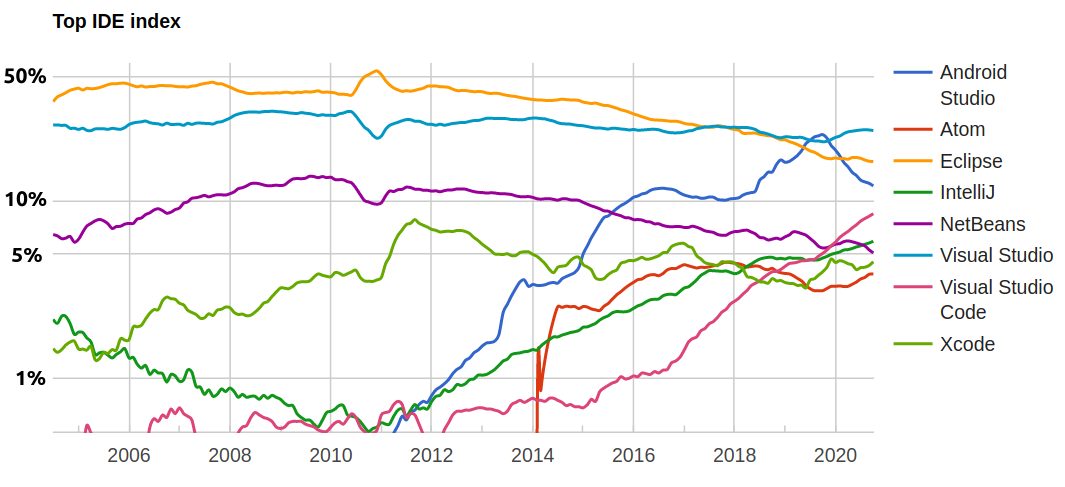
\includegraphics[width=\textwidth]{img/ide2020.png}
	\end{center}
	\centering
	Dati da \url{https://pypl.github.io/IDE.html}
\end{frame}

\section{Eclipse IDE per Java}

\begin{frame}{Eclipse IDE}
\begin{center}

\includegraphics[width=\textwidth]{img/eclipse-web-site.png}
\url{https://www.eclipse.org/}
\end{center}
\end{frame}

\begin{frame}{Eclipse IDE}
\begin{block}{Overview}
\begin{itemize}
\item Eclipse è un IDE open-source scritto in Java
\item Disponibile per diverse piattaforme (Windows, Linux, Mac OSX, ..)
\item \dots e sotto forma di diverse distribuzioni 
\begin{itemize}
\item Standard, per sviluppatori J2EE/C/C++/Python/Web, \dots
\end{itemize}
\end{itemize}
\end{block}
\vfill
\begin{block}{Un po' di storia\dots}
\begin{itemize}
\item Nato nei laboratori di ricerca IBM (alphaWorks) 
\item	Successivamente	donato alla comunità open-source che ora ne cura lo sviluppo per mezzo di un'apposita fondazione
\item Correntemente supportato/utilizzato da un vasto numero di sviluppatori, sia in ambito accademico che industriale
\end{itemize}
\end{block}
\end{frame}

\subsection{Astrazioni di Base}

\begin{frame}{Astrazioni di base in Eclipse (1/5)}
\begin{block}{Workspace}
\begin{itemize}
\item Directory in cui Eclipse salva le ``\emph{preferenze di una specifica sessione di lavoro}''
\begin{itemize}
\item Le configurazioni dell'ambiente
\item L'elenco dei progetti coinvolti
\item View e Perspective aperte/disponibili
\item Stato dei plugin installati
\item \dots
\end{itemize}
\item Memorizza tutte le informazioni d'interesse nella directory \emph{.metadata}
\item Tipicamente contiene anche i progetti (che possono però anche essere importati da altre directory)
\begin{itemize}
\item In questo caso, i progetti sono inseriti ciascuno in una directory dedicata allo stesso livello di \emph{.metadata}
\end{itemize}
\end{itemize}
\end{block}
\end{frame}

\begin{frame}{Gestione del Workspace}
\begin{itemize}
\item Il workspace d'interesse deve essere creato/scelto all'avvio di Eclipse
\end{itemize}
\begin{center}
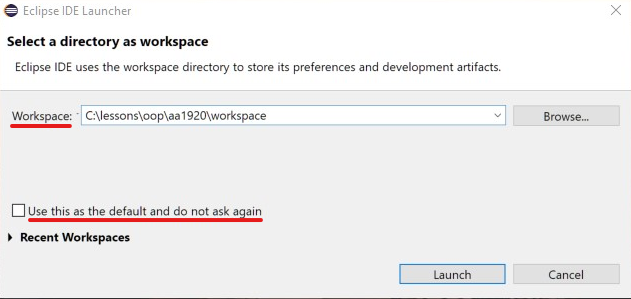
\includegraphics[width=0.8\textwidth]{img/eclipse-screenshots/eclipse-ide-00.png}
\end{center}
\begin{itemize}
\item Può essere cambiato anche dopo
\begin{itemize}
\item File $>$ Switch Workspace $>$ \dots
\end{itemize}
\end{itemize}
\end{frame}

\begin{frame}{Primo avvio}
\begin{center}
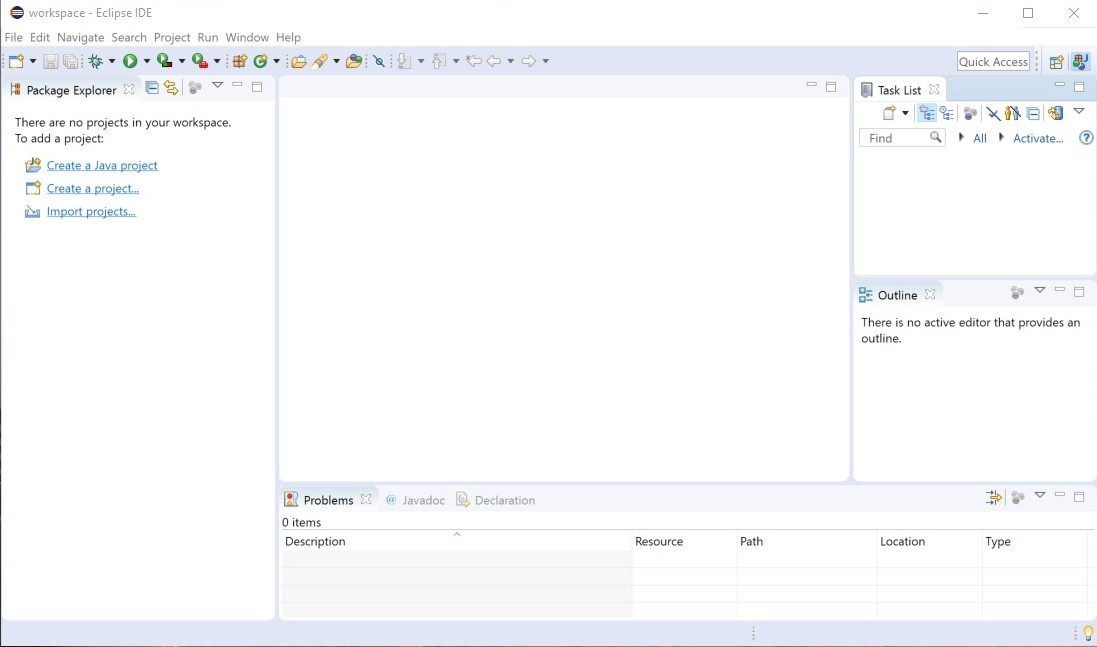
\includegraphics[width=\textwidth]{img/eclipse-screenshots/eclipse-ide-01.jpg}
\end{center}
\end{frame}

\begin{frame}{Astrazioni di base in Eclipse (2/5)}
\begin{block}{View}
\begin{itemize}
\item Componente dell'interfaccia di Eclipse
\item Tipicamente numerose view sono aperte contemporaneamente;
\item Ciascuna offre una micro-funzionalità, ad esempio:
\begin{itemize}
\item Package Explorer --- fornisce una vista dei progetti e della loro struttura;
\item Console --- consente di usare un terminale interno all'IDE invece del terminale di sistema;
\item Outline --- mostra un riassunto dei componenti della classe attualmente aperta, elencando i membri, consentendo di filtrarli (ad esempio, nascondendo i privati) e di ordinarli (ad esempio in ordine alfabetico);
\item Problems --- elenca gli eventuali problemi che affliggono il progetto (errori di configurazione, sorgenti che non compilano, warnings...)
\end{itemize}
\end{itemize}
\end{block}
\end{frame}

\begin{frame}{Astrazioni di base in Eclipse (3/5)}
\begin{block}{Perspective}
\begin{itemize}
\item Insieme di view opportunamente organizzate
\begin{itemize}
\item Cambiare perspective consente di cambiare rapidamente le view attive
\item Tipicamente, si usano perspective diverse per fasi diverse dello sviluppo
\end{itemize}
\item Ne vedremo sicuramente due:
\begin{itemize}
\item Java --- per lo sviluppo di applicazioni Java
\item Debug --- per il debug di applicazioni (prossima lezione!)
\end{itemize}
\end{itemize}
\end{block}
\end{frame}

\begin{frame}{Astrazioni di base in Eclipse (4/5)}
\begin{block}{Progetto}
\begin{itemize}
\item Directory contenente una collezione di risorse opportunamente organizzate, tipicamente rappresentanti un software o una parte di un software
\begin{itemize}
\item codice sorgente
\item file di configurazione
\item risorse (immagini, video, \dots)
\item file compilati (bytecode, in java)
\item librerie esterne
\item \dots
\end{itemize}
\item Ciascun progetto fa generalmente riferimento ad uno specifico linguaggio di programmazione
\item Ogni progetto, a seconda della propria tipologia, può utilizzare diversi strumenti per la gestione delle proprie risorse
\end{itemize}
\end{block}
\end{frame}

\begin{frame}{Creazione di un Progetto Java}
\begin{itemize}
\item File $>$ New $>$ Java Project
\end{itemize}
\begin{center}
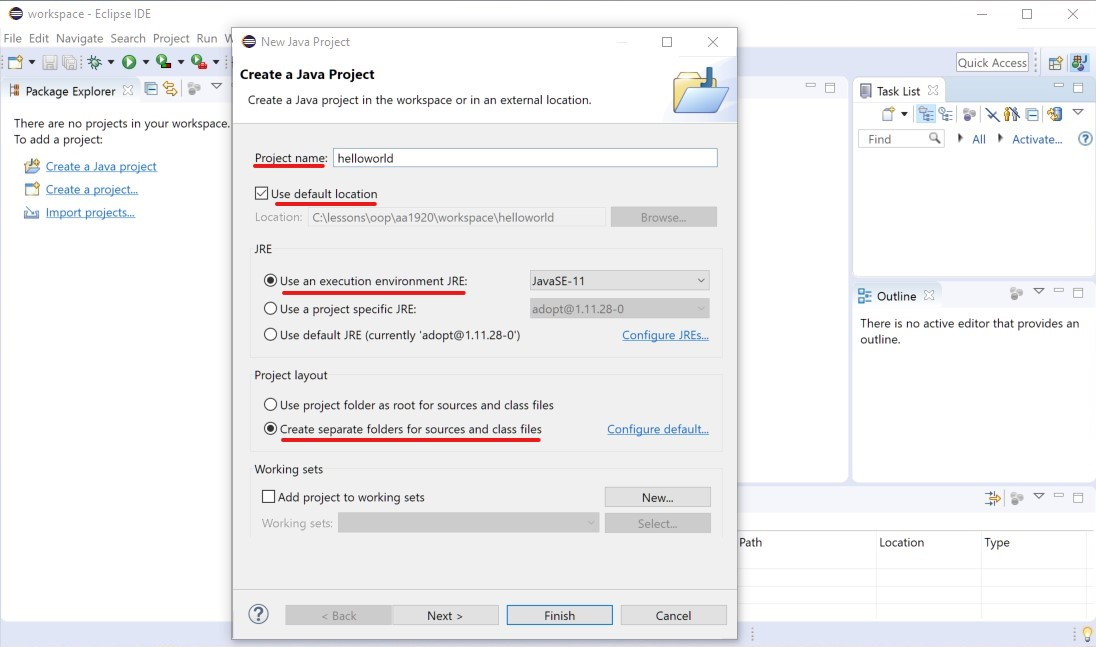
\includegraphics[width=0.9\textwidth]{img/eclipse-screenshots/eclipse-ide-02a.jpg}
\end{center}
\begin{itemize}
\item $\rightarrow$ Finish
\end{itemize}
\end{frame}

\begin{frame}{Creazione di un Progetto Java (nota sui moduli)}
\begin{itemize}
\item Nell'ambito del corso, il concetto di \emph{Modulo} non è utilizzato
\begin{itemize}
\item Per ogni nuovo progetto è quindi necessario evitare la creazione\dots
\end{itemize}
\end{itemize}
\begin{center}
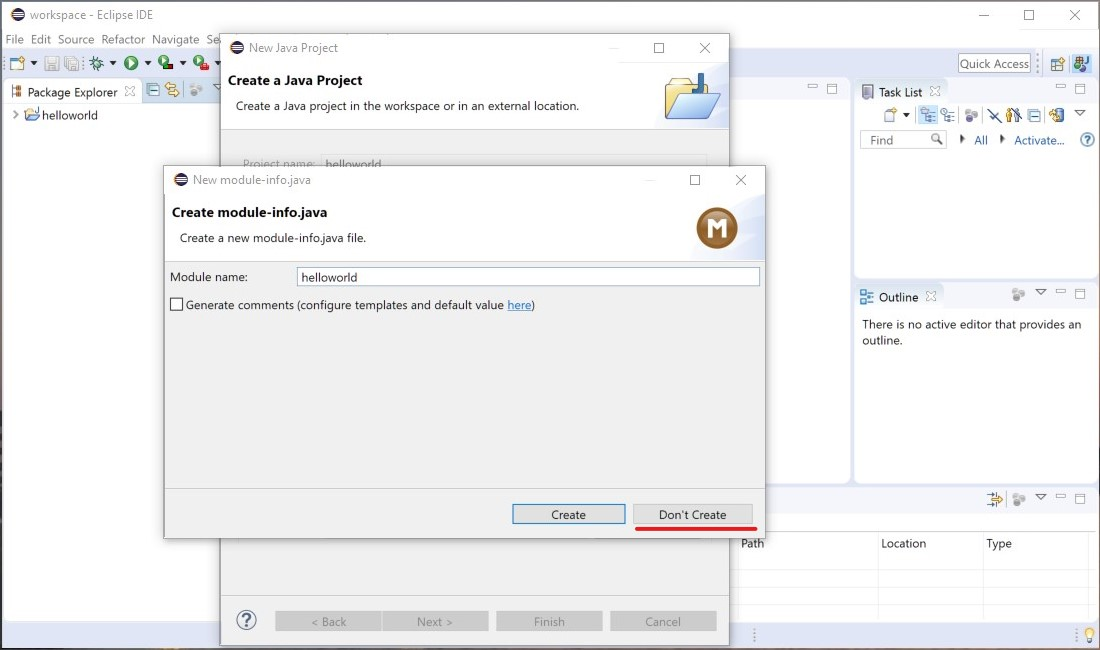
\includegraphics[width=0.9\textwidth]{img/eclipse-screenshots/eclipse-ide-02b.jpg}
\end{center}
\end{frame}

\begin{frame}{Creazione di Package e Classi}
\begin{itemize}
\item File $>$ New $>$ Package
\end{itemize}
\begin{center}
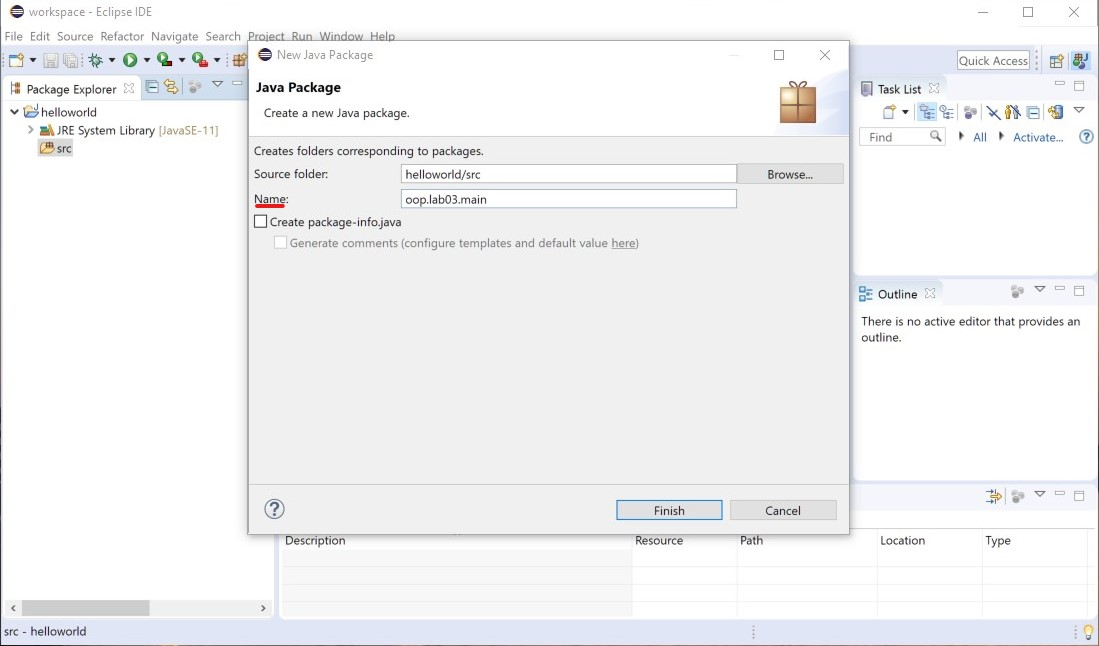
\includegraphics[width=0.9\textwidth]{img/eclipse-screenshots/eclipse-ide-02c.jpg}
\end{center}
\end{frame}

\begin{frame}{Creazione di Package e Classi}
\begin{itemize}
\item (click dx su package in Package Explorer View) $>$ New $>$ Class
\end{itemize}
\begin{center}
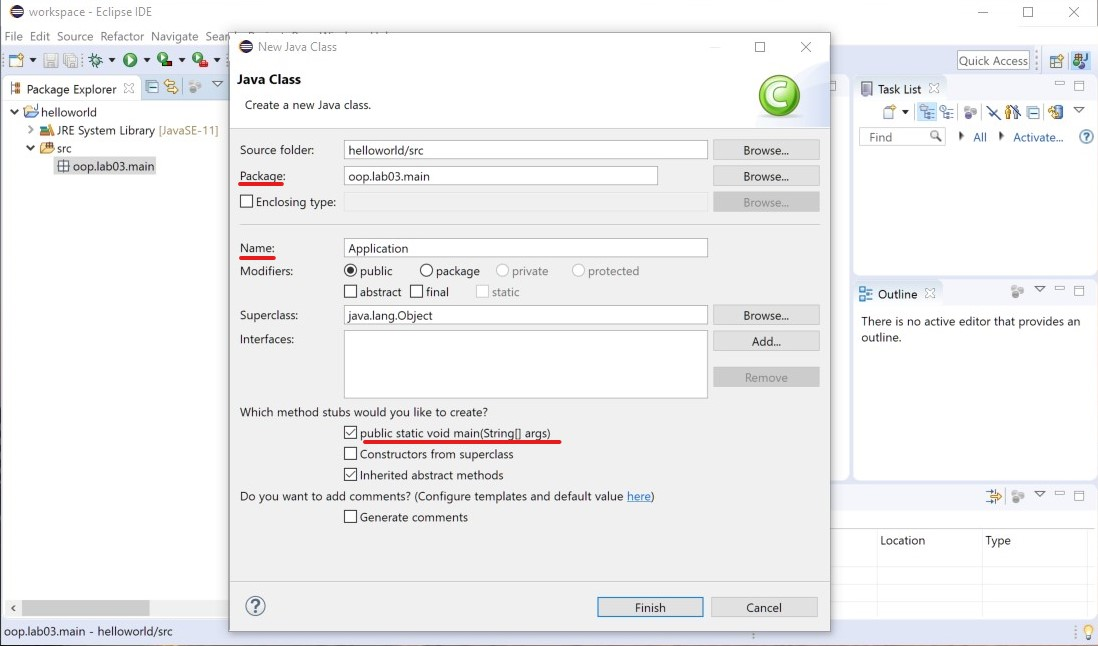
\includegraphics[width=0.9\textwidth]{img/eclipse-screenshots/eclipse-ide-02d.jpg}
\end{center}
\end{frame}

\begin{frame}{JDT: Code Completion e Syntax Highlighting}
\begin{center}
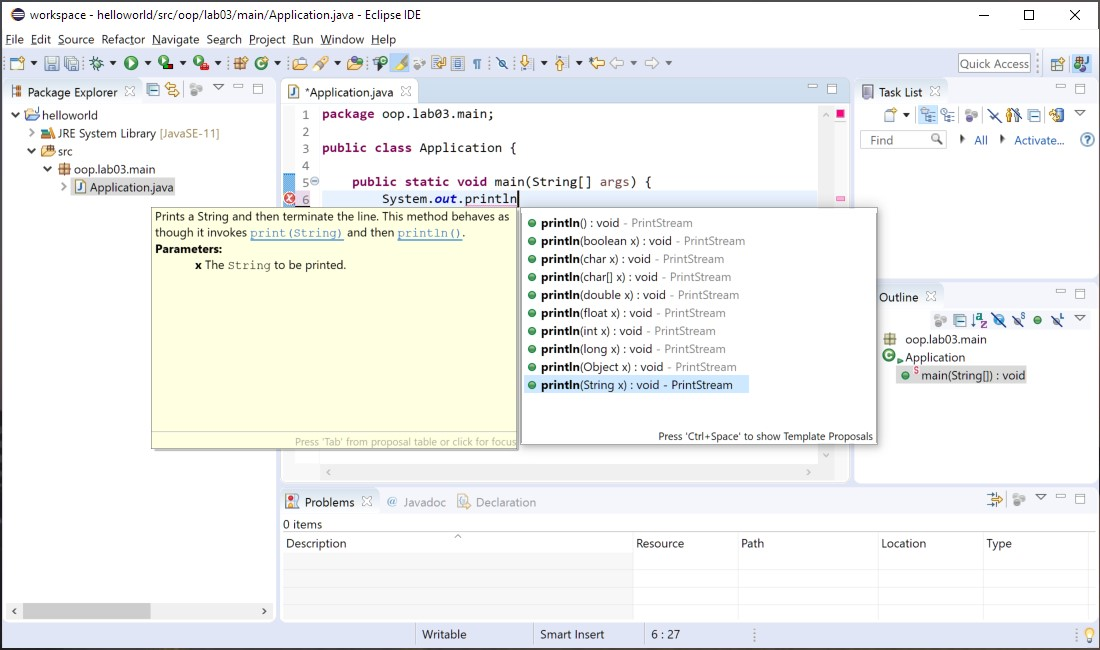
\includegraphics[width=0.85\textwidth]{img/eclipse-screenshots/eclipse-ide-03.jpg}
\end{center}
\begin{itemize}
\item CTRL+Space : richiama la code completion su una porzione di codice
\end{itemize}
\end{frame}

\begin{frame}{Compilazione dei Sorgenti}
\begin{center}
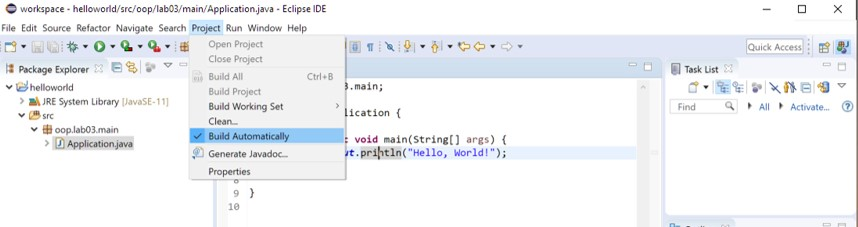
\includegraphics[width=0.9\textwidth]{img/eclipse-screenshots/eclipse-ide-04a.jpg}
\end{center}
\begin{block}{Due diverse possibilità}
\begin{itemize}
\item \textbf{Compilazione automatica}
\begin{itemize}
\item Il compilatore viene invocato automaticamente dall'IDE ad ogni modifica (salvata) ai sorgenti del progetto
\item E' la modalità che generalmente è da preferire
\end{itemize}
\item \textbf{Compilazione manuale}
\begin{itemize}
\item Attiva solo quando è disabilitata la compilazione automatica
\item Il compilatore viene invocato a seguito di un esplicito click dello sviluppatore su \textit{``Build All''} (CTRL+B)
\end{itemize}
\end{itemize}
\end{block}
\end{frame}

\begin{frame}{Esecuzione di Applicazioni}
\begin{itemize}
\item (click dx su classe principale) $>$ Run As $>$ Java Application
\end{itemize}
\begin{center}
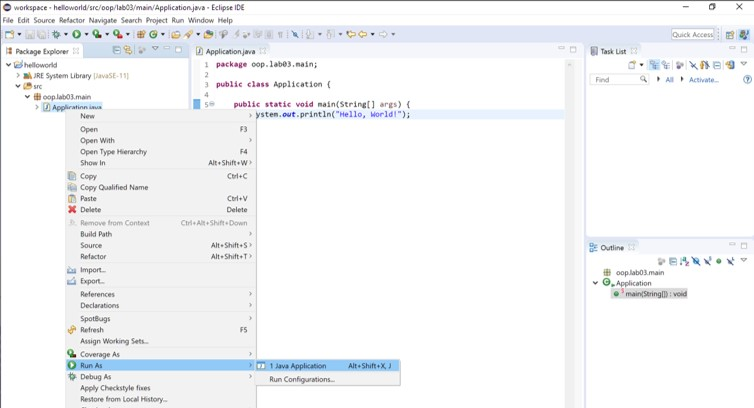
\includegraphics[width=0.9\textwidth]{img/eclipse-screenshots/eclipse-ide-04b.jpg}
\end{center}
\end{frame}

\begin{frame}{Esecuzione di Applicazioni -- Output View}
\begin{center}
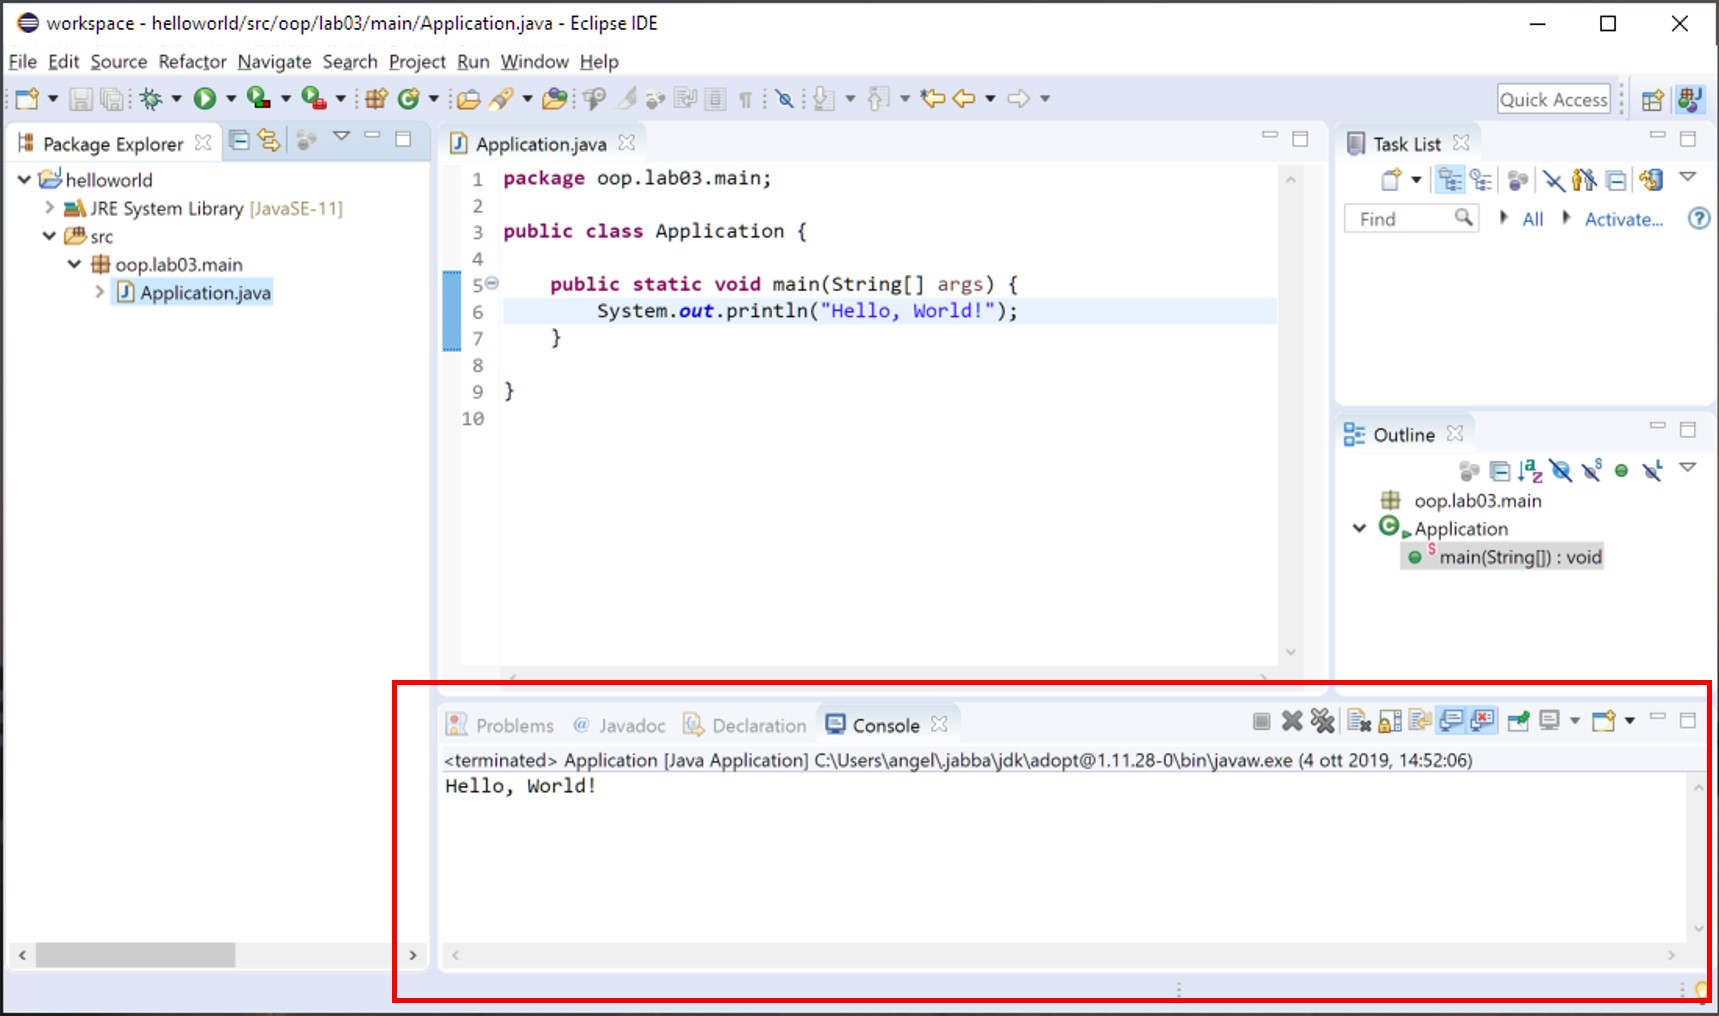
\includegraphics[width=\textwidth]{img/eclipse-screenshots/eclipse-ide-04c.jpg}
\end{center}
\end{frame}

\begin{frame}{Run Configuration}
\begin{itemize}
\item Consente di personalizzare la configurazione con la quale l'applicazione va in esecuzione
\begin{itemize}
\item Ad esempio, i parametri da passare in ingresso al metodo main
\end{itemize}
\item Run $>$ Run Configurations
\end{itemize}
\begin{center}
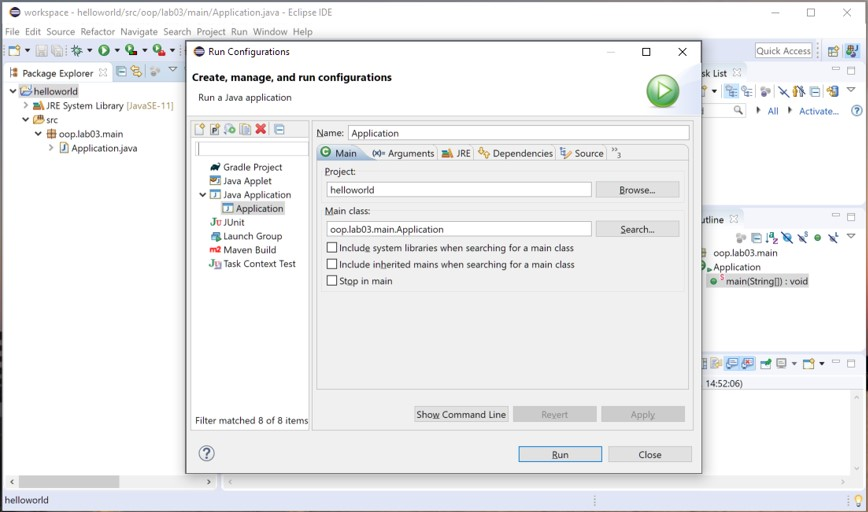
\includegraphics[width=0.8\textwidth]{img/eclipse-screenshots/eclipse-ide-04d.jpg}
\end{center}
\end{frame}

\begin{frame}{Run Configuration: Program Arguments}
\begin{center}
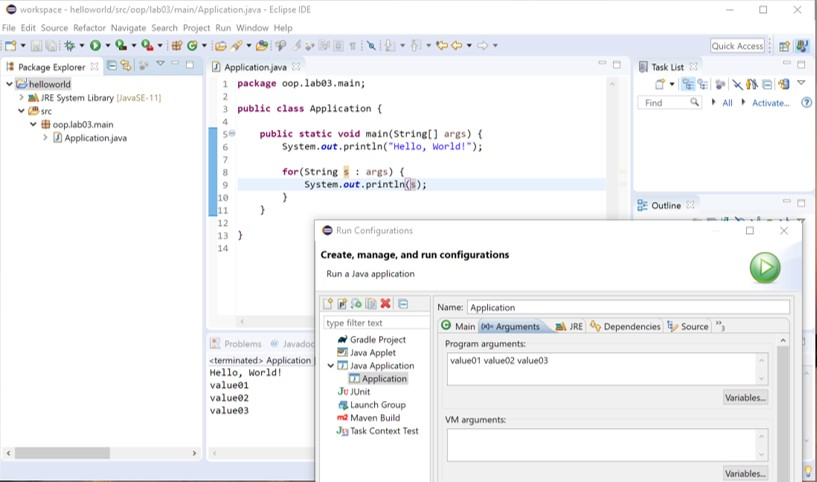
\includegraphics[width=\textwidth]{img/eclipse-screenshots/eclipse-ide-04e.jpg}
\end{center}
\end{frame}

\begin{frame}{Java Build Path}
\begin{itemize}
\item (click dx su progetto) $>$ Build Path $>$ Configure Build Path
\end{itemize}
\begin{center}
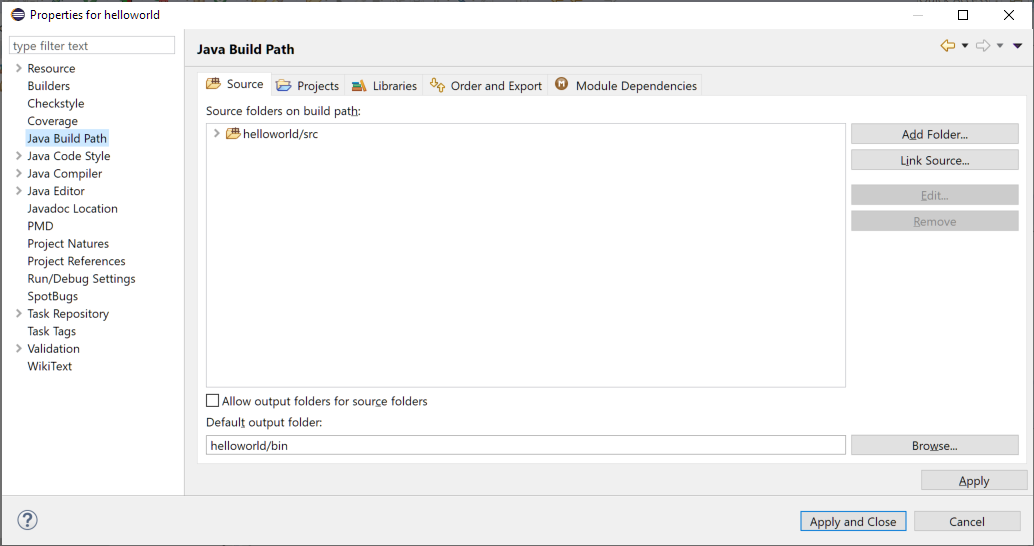
\includegraphics[width=\textwidth]{img/eclipse-screenshots/eclipse-ide-05a.png}
\end{center}
\end{frame}

\begin{frame}{Java Project Resources}
\begin{itemize}
\item (click dx su progetto) $>$ Properties $>$ Resource
\end{itemize}
\begin{center}
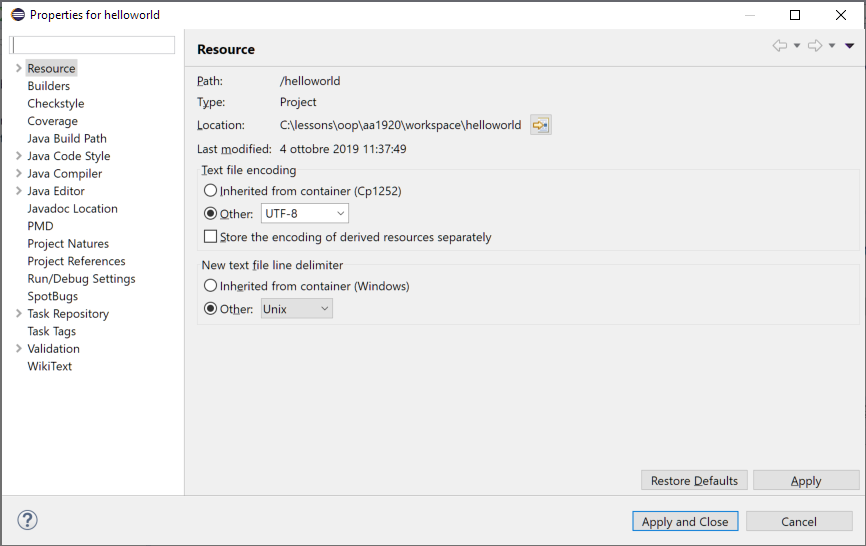
\includegraphics[width=0.7\textwidth]{img/eclipse-screenshots/eclipse-ide-05b.png}
\end{center}
\textbf{Importante}:
\begin{itemize}
\item Text File Encoding: UTF-8
\item New text file line Delimiter: Unix
\end{itemize}
\end{frame}

\begin{frame}{Importazione di Progetti Esistenti (1/2)}
\begin{itemize}
\item File $>$ Import\dots $>$ General $>$ Existing Project Into Workspace
\end{itemize}
\begin{center}
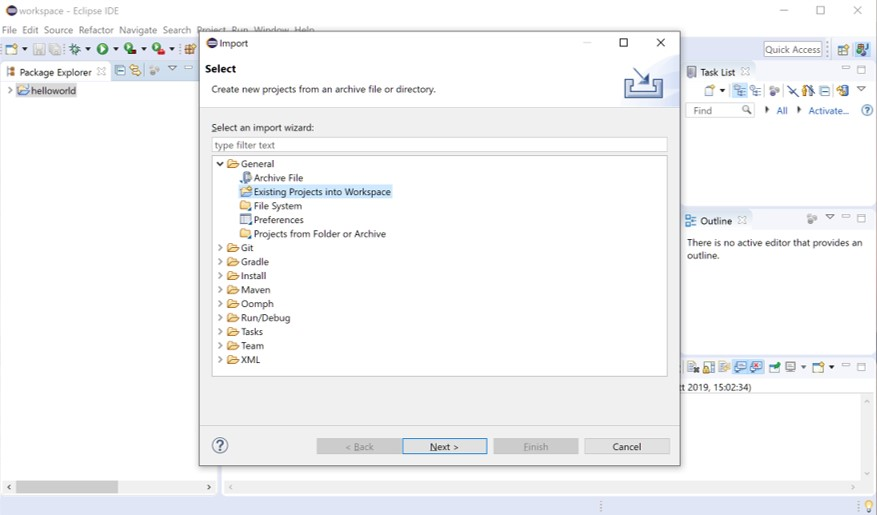
\includegraphics[width=\textwidth]{img/eclipse-screenshots/eclipse-ide-06a.jpg}
\end{center}
\end{frame}

\begin{frame}{Importazione di Progetti Esistenti (2/2)}
\begin{itemize}
\item Selezionare la directory del progetto
\begin{itemize}
\item Generalmente, una directory di un progetto Java importabile in Eclipse contiene almeno i file \emph{.project}, \emph{.classpath} e la directory \emph{.settings}, oltre ai sorgenti del progetto.
\end{itemize}
\item Decidere se copiare il progetto nel workspace oppure se continuare a modificare il progetto nella sua posizione originale sul filesystem
\end{itemize}
\begin{center}
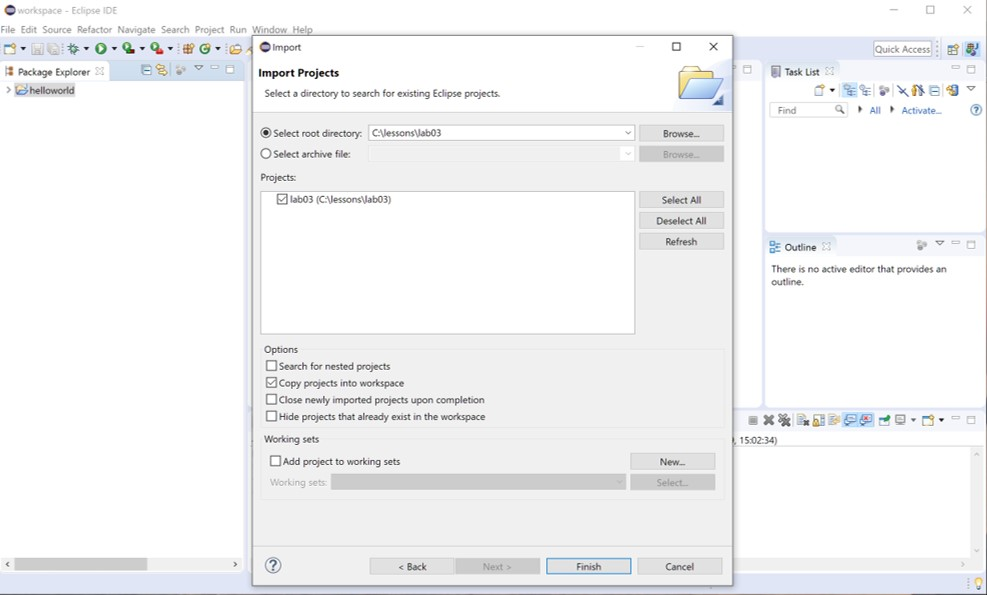
\includegraphics[width=\textwidth]{img/eclipse-screenshots/eclipse-ide-06b.jpg}
\end{center}
\end{frame}

\begin{frame}{Astrazioni di base in Eclipse (5/5)}
\begin{block}{Plug-in}
Software installabile opzionalmente che estende le capacità dell'IDE, ad esempio:
\begin{itemize}
\item controllare la qualità del codice Java;
\item aggiungere supporto ad ulteriori linguaggi;
\item usare sistemi di build diversi da quello predefinito (Gradle, Maven...);
\end{itemize}
\end{block}

\begin{itemize}
\item Ne vedremo diversi durante il corso\dots
\end{itemize}
\end{frame}


%\subsection{Architettura}
%
%\fr{Eclipse Architecture}{
%	
%	\bl{Eclipse ha una architettura organizzata a plug-in}{
%		\iz{
%			\item Un plug-in è un modulo (classi + meta-informazioni + manifest file) auto-contenuto che incapsula una certa funzionalità
%				\iz{
%						\item File editor specifici, wizard, build, compilazione e debugging di sorgenti
%						\item Costituisce l'unità funzionale elementare dell'architettura
%				}
%			\item Possono essere definite relazioni di dipendenza, composizione, etc. specifiche dell'astrazione plug-in (non parte dell'OOP)
%				\iz{
%					\item Non le tratteremo nel dettaglio in questo corso
%				}
%		}
%	}
%	
%	\bl{Eclipse come IDE Modulare}{
%		\iz{
%			\item Nuovi plug-in possono essere liberamente installati al bisogno
%				\iz{
%					\item Ne esistono moltissimi open-source, altri sviluppati da aziende e università
%				}
%			\item Supporto nativo lo sviluppo di nuovi plug-in
%				\iz{
%					\item Plug-in Development Environment (PDE)
%				}
%		}
%	}
%}
%
%
%\fr{Plug-in and Perspective}{
%
%	\bl{Che relazione tra plug-in e perspective?}{
%		\iz{
%			\item Le prospettive disponibili sono definite dai plug-in installati
%			\item Prospettive disponibili di default (e.g. Resource, Java, Debug, Git,..)
%		}
%	}
%	\bl{Descrizione di alcune delle perspective di default}{
%		\iz{
%			\item \textcolor{blue}{Resource perspective}: permette di navigare e interagire con le risorse in termini di file
%				\iz{
%					\item  Il progetto è visto come una collezione di file e directory, che è possibile creare, modificare, spostare, etc.
%				}
%		
%			\item \textcolor{blue}{Java perspective}: fornisce viste ed editor per gestire tutte le attività più significative per lo sviluppo di progetti Java
%				\iz{
%					\item Realizzata da un insieme di plug-in che prendono il nome di JDT (Java Development Tools)
%				}
%
%			\item ...
%			
%		}
%	}
%}
%
%\fr{Resource Perspective (Default Perspective)}{
%		\fg{height=0.85\textheight}{img/default_perspective.png}
%}
%
%\fr{JDT e Java Perspective}{
%		\fg{height=0.85\textheight}{img/jdt_perspective.png}
%}


\subsection{Refactoring}

\begin{frame}{Refactoring}
	\begin{block}{}
		\emph{Refactoring is a disciplined technique for restructuring an existing body of code, 
altering its internal structure without changing its external behavior.}\\--- \url{refactoring.com}
	\end{block}
	\begin{block}{Vantaggi nel refactoring supportato dall'IDE}
		\begin{itemize}
			\item Le modifiche sono gestite dall'IDE in maniera consistente
			\begin{itemize}
				\item \footnotesize{Es (1). \emph{Rinominare una variabile}: se si procede ``a 
mano'', si dovrà modificare il nome della variabile sia nella riga in cui la si dichiara sia in 
tutte le sue occorrenze di utilizzo. Viceversa, avvalendosi dell'IDE, la modifica da fare è una 
sola.}
				\item \footnotesize{Es (2). \emph{Spostare una classe da un package ad un altro}: 
utilizzando l'IDE vengono aggiornati tutti i riferimenti nell'intero progetto}
			\end{itemize}
			\item Minimizza l'introduzione di errori in fase di refactoring
		\end{itemize}
	\end{block}
\end{frame}

\fr{Refactoring in Eclipse}{
	\bl{}{
		Operazioni di modifica del nome di variabili, classi, metodi etc.
		\iz{ 
			\item Gestite in maniera automatica e safe dall'IDE 
			\item Attivabile anche tramite ALT+SHIFT+R sulla selezione di interesse
		}
	}
	\fg{height=0.7\textheight}{img/refactor.png}
}

\subsection{Keyboard Shortcuts}

\begin{frame}{Keyboard Shortcuts}
\begin{itemize}
\item \alert{CTRL+1}: quick-fix contestuale per errori (molto potente)
\item \alert{ALT+SHIFT+R}: refactoring di campi/metodi/classi
\item \alert{CTRL+SHIFT+/}: commento delle linee selezionate
\item \alert{CTRL+PGUP/PGDOWN}: per muoversi di uno step avanti (PGUP) o indietro 
(PGDOWN) tra la lista di sorgenti correntemente aperti
\item \alert{F3} (o \alert{CTRL+CLICK}): ci sposta alla definizione di un dato elemento 
\item \alert{CTRL+SHIFT+L}: lista delle shortcut disponibili per il dato contesto 
\item \alert{CTRL+SHIFT+O}: include in automatico tutti gli import necessari sulla base 
delle classi utilizzate nel sorgente corrente
\item \alert{CTRL + . }: sposta il cursorse al successivo errore/warning
\item \alert{CTRL+F8}: consente di spostarsi tra le varie perspective
\item \alert{CTRL+J}: search incrementale, senza l'uso di GUI
\item \alert{ALT+SHIFT+S}: da l'accesso a un insieme di wizard con cui automatizzare la 
scrittura di costruttori, getter, setter, etc.
\end{itemize}
\end{frame}

\section{Debugging di Applicazioni}

\begin{frame}[allowframebreaks]{Debugging di Applicazioni \cite{debugger,debugging}}
	\begin{block}{Motivazioni}
		\begin{itemize}
			\item Difficilmente le applicazioni software risultano essere totalmente esenti da 
problemi/errori alla prima stesura del codice sorgente
			\item Spesso lo sviluppatore tende a sottovalutare e/o ignora alcuni effetti collaterali 
(\emph{side-effects}) che porzioni di codice sorgente possono provocare
			\item In genere, un software privo di errori lo si ottiene step-by-step
			\begin{itemize}
				\item Una buona progettazione a priori consente di ridurre il numero di bug che si 
potrebbero inserire nel codice sorgente, tuttavia\dots
				\item \dots qualche bug sarà inevitabilmente presente, e dovrà essere identificato e 
corretto!
			\end{itemize}
		\end{itemize}
	\end{block}
	\begin{block}{Approcci}
		\begin{enumerate}
			\item \textcolor{blue}{Meccanismi di logging}
			\begin{itemize}
				\item Si aggiunge al codice sorgente la possibilità di fare logging in modo da 
tracciare lo stato interno del programma in fase di esecuzione: valore corrente di variabili, campi, 
parametri, \dots
				\item Utile in alcuni casi, ma in generale \textbf{da evitare}!
				\item Appesantisce il sorgente
				\item Appesantisce il software (a meno di non usare opportune librerie)
				\item Basta un side effect per generare un Heisenbug \cite{heisenbug}
			\end{itemize}
			\item \textcolor{blue}{Utilizzo di strumenti di debugging forniti dall'IDE}
			\begin{itemize}
				\item Controllo efficace sull'esecuzione dell'applicazione
				\item Ispezionabilità a run-time
				\item Potenti strumenti per indagare cosa succede nel programma
				\item Molto difficile che causi Heisenbugs
				\begin{itemize}
					\item Finché non si mette in mezzo la concorrenza...
				\end{itemize}
			\end{itemize}
		\end{enumerate}
	\end{block}
\end{frame}

\begin{frame}[allowframebreaks]{Debug: concetti principali}
    \begin{block}{Breakpoint}
        Speciale punto di controllo che, se raggiunto dal flusso di controllo, sospende l'esecuzione
    \end{block}
    \begin{block}{Espressioni e osservabilità}
        La capacità valutare espressioni che includono variabili attualmente accessibili dal 
flusso di controllo, osservandone il valore corrente
    \end{block}
    \begin{block}{Modifica dei valori a tempo d'esecuzione}
        La capacità modificare i valori di variabili e campi manualmente a programma in esecuzione, 
una volta che il flusso di controllo è sospeso
    \end{block}
    \begin{block}{Step-by-step execution}
        La capacità, a flusso di lavoro sospeso (e, quindi, una volta incontrato un breakpoint) di 
proseguirla andando avanti di un'istruzione alla volta
    \end{block}
    \begin{block}{Step-into execution}
        La capacità, a flusso di lavoro sospeso (e, quindi, una volta incontrato un breakpoint) di 
proseguirla ``entrando'' nel record di attivazione di un metodo che viene invocato
    \end{block}
\end{frame}


\fr{Debugging di Applicazioni in Eclipse}{
\iz{
\item L'avvio del debugging è molto simile all'esecuzione delle applicazioni
\iz{\item (menu contestuale di progetto) $>$ Debug As $>$ Java Application
}
}
\fg{height=0.7\textheight}{img/debug.png}
}


\fr{Debugging in Eclipse: manipolazione del flusso di controllo}{
	\iz{
		\item L'avvio del debugger in Eclipse comporta l'apertura della perspective \emph{Debug}, 
con gli strumenti utili per le operazioni di debugging
	}
	\bl{Principali operazioni di manipolazione del flusso di controllo}{
		\en{
			\item Inserimento di un breakpoint
			\iz{
				\item Doppio click sulla linea di interesse (o CTRL+SHIFT+B)
			}
			\item Esecuzione \textcolor{blue}{step-by-step}: F6
			\iz{
				\item Una volta che l'esecuzione è stata sospesa da un breakpoint
			}
			\item \textcolor{blue}{Step into}: F5 
			\iz{
				\item Debugging corpo di un metodo/costruttore
			}
				\item \textcolor{blue}{Step return}: F7 
			\iz{
				\item Ritorno dal debugging del corpo di un metodo/costruttore
			}
			\item \textcolor{blue}{Resume}: F8 
			\iz{
				\item Esecuzione fino al prossimo breakpoint 
			}
		}
	}
}

\begin{frame}[allowframebreaks]{Debugging in Eclipse: strumenti}
	\begin{block}{Breakpoint condizionali}
		Tramite click destro su breakpoint e ``Properties'', è possibile scrivere una condizione per 
il breakpoint, ad esempio di scattare solo dopo un certo numero di volte, oppure di scattare se una 
certa condizione è vera (estremamente utile).
	\end{block}
	\begin{block}{Osservazione e manipolazione dei valori}
		La view ``Variables'' consente di visualizzare il valore di tutti i campi e delle variabili 
locali, esplorando anche l'interno degli oggetti. Inoltre, consente di modificarne i valori a 
runtime, per ispezionare il funzionamento del programma.
	\end{block}
	\begin{block}{Valutazione di espressioni}
		È possibile, nella tab ``Expressions'', scrivere un'espressione java valida nel contesto 
(quindi, con accesso alle variabili locali e ai campi). L'IDE la valuterà e scriverà il risultato. 
Molto utile per visualizzare valori che richiederebbero altrimenti l'inserimento di una stampa ed il 
riavvio del debug, oppure un uso complicato dell'osservazione dentro Variables.
	\end{block}
%	\begin{block}{Iniezione di codice a caldo}
%		Nel caso in cui si effettui una modifica al software mentre è in esecuzione in modalità 
%debug e lo si ricompili (o si abbia la modalità di autocompilazione attivata), Eclipse tenterà di 
%``iniettare'' i nuovi compilati all'interno della JVM in esecuzione:
%		\begin{itemize}
%			\item Viene ``scaricata'' la classe precedentemente inserita nel classpath
%			\item Viene ``iniettata'' la nuova classe
%		\end{itemize}
%		L'operazione può fallire, nel qual caso l'IDE notificherà che ci sono in esecuzione classi e 
%metodi obsoleti. Per massimizzare la riuscita:
%		\begin{enumerate}
%			\item Scegliere uno stack frame precedente all'uso della classe da sostituire;
%			\item Usare la funzione ``Drop to frame'' per riportare il flusso di controllo 
%all'inizio dello stack frame che si sta eseguendo;
%			\begin{itemize}
%				\item Eventuali side effects non vengono cancellati!
%				\item (altro esempio in cui l'immutabilità è d'aiuto)
%			\end{itemize}
%			\item Solo a questo punto salvare il sorgente modificato.
%		\end{enumerate}
%	\end{block}
\end{frame}

\section{Lab Startup}

\begin{frame}[allowframebreaks]{Preparazione ambiente di lavoro}
    \begin{itemize}
        \item Collegarsi al sito del corso
        \item Scaricare il file zip contenente gli esercizi del laboratorio
        \item Decomprime la directory sul Desktop
        \item Aprire Eclipse
        \item Eseguire la procedura di importazione del progetto esistente
    \end{itemize}
\end{frame}

\fr{Modalità di Lavoro}{
	\bl{}{
		\en{
			\item Leggere la consegna
			\item Risolvere l'esercizio in autonomia
			\item Cercare di risolvere autonomamente eventuali piccoli problemi che possono verificarsi durante lo svolgimento degli esercizi
			\item \alert{Utilizzare le funzioni di test presenti nei sorgenti per il testing dell'esercizio}
			\item Contattare i docenti nel caso vi troviate a lungo bloccati nella risoluzione di uno specifico esercizio
			\item A esercizio ultimato contattare i docenti per un rapido controllo della soluzione realizzata
			\item Proseguire con l'esercizio seguente
		}
	}
}

\begin{frame}[allowframebreaks]
 \frametitle{Bibliography}
  \bibliographystyle{plain}
  \small
 \bibliography{biblio}
\end{frame}

\end{document}
